\setstretch{1.3}
\chapter{Spontaneous Symmetry Breaking of the Lugiato-Lefever Equation}
\label{chap:LL}
\lhead{Chapter 4. \emph{SSB of the LL Equation}}

\setstretch{2}
The following chapter is based on Ref.~\cite{JuliaSSB} coauthored with Ricardo Carretero-Gonz\'alez, Panayotis G. Kevrekidis, and Mariana Haragus.  The aim of the chapter is to further extend the NCVA approach to a variant of the NLS equation: the mean-field Lugiato-Lefever (LL) 
model~\cite{LL,LLE}.  Experimentally~\cite{XuCoen}, temporal spontaneous symmetry breaking (SSB) is found in passive Kerr resonators described by the LL equation.  We examine this SSB-induced 
instability interval in the the passive 
Kerr resonator modeled by the Lugiato-Lefever equation %Eq.~(\ref{NLSEq})
by means of the NCVA~\cite{JuliaNCVA} described in Chapter~\ref{chap:NCVA}, and further through
a center manifold reduction~\cite{MH-Iooss}
enabling the analysis of the dominant associated eigenmodes (responsible
for determining the spectral stability of the system).  
It is relevant to mention at this point that a thorough  bifurcation analysis for a LL equation in the case of constant external pumping
was recently carried out in Ref.~\cite{LLE_french_PRA}, showing quite complex bifurcation scenarios in both the anomalous and normal dispersion regimes.
%
In the NCVA context, our aim is to
apply a variational method based on well-informed ans\"{a}tze 
in the corresponding
Lagrangian of the system.  The ans\"{a}tze reduce the complexity of the 
original 
infinite-dimensional problem to a few degrees of freedom capturing the 
principal,
static and dynamic characteristics of the system.  
%
This method attempts to project the infinite-dimensional dynamics of the Lugiato-Lefever equation 
%Eq.~\ref{NLSEq} 
into a low-dimensional dynamical system that qualitatively and, to some
extent, quantitatively captures SSB bifurcations an the solutions emanating from it.
%
%However, it is important to note that traditional variational methods rely on the 
%existence of a Lagrangian or Hamiltonian structure for closed systems for which 
%equations of motion can be derived. Nonetheless, recently, 
Based on Galley's~\cite{Galley} approach to extend variational approximation method to open, non-conservative dissipative systems we developed the NCVA,  
which in turn was generalized to dissipative (containing gain and loss) NLS-type
systems in Ref.~\cite{JuliaNCVA}.  This was inspired by the work of Ref.~\cite{ref4} on the 
extension of Galley's formalism to ${\mathcal PT}$-symmetric variants of field theories. It is this variant of the NCVA that we will explore in the present
setting.

The chapter is organized as follows.
%
In Sec.~\ref{section:SSB} we introduce SSB and setup the LL model.  In Sec.~\ref{secModel} we identify the equilibria and study their stability by means 
of a spectral analysis of the linearization problem; this is a perspective
that was absent in the original work of Ref.~\cite{XuCoen} and which, we 
argue, provides a more systematic insight into the stability (and the
potential instabilities) of the system. 
In doing so, we recover the forward and reverse 
pitchfork bifurcations (i.e., a pitchfork loop) observed in Ref.~\cite{XuCoen} as well 
as identify a Hopf bifurcation for larger pump power giving rise to asymmetric,
stable, periodic solutions; the latter is an important feature of 
dynamical interest
in its own right.
%
%Section~\ref{secNCVA} is devoted to the NCVA approach.
%In Sec.~\ref{secNCVA:prelim} we provide a brief description of the 
%NCVA approach and its formulation within the LL model.
%
Section~\ref{secNCVA:app} is devoted to the application of the NCVA to capture
the SSB bifurcation for physically relevant parameters values of the system 
as in Ref.~\cite{XuCoen}.
%
In Sec.~\ref{secGalerkin} we complement our understanding of the pitchfork
loop bifurcation by giving the local bifurcation analysis which is effective 
towards qualitatively and quantitatively describing the emerging asymmetric solutions
close to the pitchfork bifurcation points. 
%
Finally, in Sec.~\ref{secConclusion} we summarize
our findings.
% and we provide possible
%avenues for future research.

\setstretch{1.3}
\section[Spontaneous Time-Reversal Symmetry Breaking in Passive Kerr Resonator]{Spontaneous Time-Reversal Symmetry Breaking in \\
Synchronously-Pumped Passive Kerr Resonators} \label{section:SSB}
\setstretch{2}
%
Spontaneous symmetry breaking (SSB) is the basis for many phase transitions and account for effects including ferromagnetism, superconductivity, and convection cells~\cite{zurek,stanley}.
%
SSB has been widely observed in nonlinear optics and is at the heart of numerous
fundamental phenomena including, but not limited to, asymmetric
dynamics in coupled 
mode models~\cite{kenkre}, optical wave guide arrays~\cite{Boris_Gisin_Kaplan_PRE_2000},
coupled nonlinear micro-cavities~\cite{Haelterman_OE_2006}, 
photonic lattices~\cite{Panos_PLA_2005}. For a detailed exposition
of numerous recent directions within the subject from the perspective
of nonlinear phenomena, see Ref.~\cite{Boris_SSB_book}.
%
SSB is not restricted to Hamiltonian (conservative) systems. For instance, 
over the past few years, it has also played a prominent role in the context of parity-time, 
so-called ${\mathcal PT}$, symmetric
systems~\cite{kivshar,yang} bearing a balanced interplay between 
gain and loss. 
%
There, it is responsible for the emergence 
%and bifurcation of solitons,
%vortices~\cite{rcg:85} and their so-called 
of novel ``ghost'' states both in the case of dimers~\cite{cartarius}, but also in that
of continuous media~\cite{rcg:88}, where they can be responsibility
for the destabilization and bifurcations associated with solitary
waves and vortices.

%in {\cal PT}-symmetric systems containing 
A remarkable example of SSB in a dissipative system was observed by 
Xu and Coen in Ref.~\cite{XuCoen} where a system using an optical fiber ring cavity composed of 
a synchronously-pumped 
passive optical resonator filled with a Kerr nonlinear material was experimentally 
explored. This system exhibits a {\em temporal} SSB instability in which the 
discrete time-reversal symmetry is broken and symmetric states become unstable
in favor of stable asymmetric states.  
%
It is the purpose of the present chapter to complement
the experimental and numerical analysis of Ref.~\cite{XuCoen} by
putting forward a thorough analytical
(and partially numerically assisted) 
understanding of the origin and manifestation of SSB bifurcations in this 
system.

We consider, as in Ref.~\cite{XuCoen}, a model for a passive Kerr resonator in an 
optical fiber ring cavity described by a single PDE,
resulting from an averaging procedure, of the NLS
equation-type, known as the mean-field Lugiato-Lefever (LL) 
model~\cite{LL,LLE}. The LL
equation, taking into account gain and loss in the system, can be cast, 
in non-dimensional form, as~\cite{XuCoen,XuCoenRef22a,XuCoenRef22b}:
%
\begin{equation}
\frac{\partial E(z, \tau)}{\partial z} = \left[ -1 + i (\left\vert E\right\vert^2 - \Delta ) - i \eta \frac{\partial^2}{\partial \tau^2} \right] E + S(\tau), 
\label{NLSEq}
\end{equation}
%
where $z$ is the slow evolution variable of the intracavity field $E$ over 
successive normalized cavity round-trips and $\tau$ describes the temporal 
%profile of 
variable in the dependence of the intracavity pulse envelope.  
%
The terms in the right-hand-side  of Eq.~(\ref{NLSEq}) correspond, respectively, to
cavity losses $(-E)$, Kerr nonlinearity $(i \left\vert E\right\vert^2 E)$, cavity 
phase detuning $(-i \Delta E)$, chromatic dispersion 
$( - i \eta \frac{\partial^2}{\partial \tau^2}E)$, and external pumping $( S(\tau))$.  
%
Within this non-dimensional form~\cite{XuCoenRef22a,XuCoenRef22b}, 
the cavity phase detuning
corresponds to $\Delta = \delta_0\alpha$, where $\alpha$ is half the fraction of 
power lost per round-trip and the cavity finesse is $\mathscr{F} = \pi/\alpha$, and 
$\delta_0 = 2m\pi  - \phi_0$ where $\phi_0$ is the overall cavity round-trip 
phase shift and $m$ is the order of the closest cavity resonance.  
%
The sign of the group-velocity dispersion coefficient of the fiber is $\eta$ 
which is taken as $\eta = -1$ for our analysis with self-focusing nonlinearity.  
The field envelope of the external pump pulses, $S(\tau)$, is modeled by a symmetric chirp-free Gaussian pulse given by $S(\tau) = \sqrt{X} \exp\left[ -(\tau/T_0)^2 \right]$,
with $T_0 = 2.3$ as in the experiments of Ref.~\cite{XuCoen}.

For the SSB instability of the passive Kerr cavity, the pump pulse field profile is temporally symmetric, $S(\tau) = S(-\tau)$, and the model is symmetric under a time reversal transformation, $\tau \rightarrow -\tau$, 
yet it admits asymmetric solutions, as described in Ref.~\cite{XuCoen}.  The 
associated pitchfork bifurcation illustrates that at low pump peak power $X$, the solutions are symmetric in time; however, above a certain pump peak power threshold the symmetric states become unstable while stable asymmetric states
emerge.  
%
The particular experimental parameters of Ref.~\cite{XuCoen} generate, as $X$ is
increased further, a reverse pitchfork as well, in which the asymmetric states
collide and disappear while the symmetric state recovers its stability.
%
%The decline in the observed $|E(\tau=0)|^2$ is caused by the peak of the 
%intracavity pulse shifting towards the right or left and breaking alignment 
%with the center of the pump pulse.
%For $\Delta = 0.92$ and $T_0=2.3$, the bifurcation point for the instability 
%is obtained at $X=4.55$ in Ref.~\cite{XuCoen}.
%
%The main aim of this manuscript is 


%%%%%%%%%% Section Stability
\subsection{The Full Lugiato-Lefever Model: Equilibria, Stability and Bifurcations
\label{secModel}}
%
In this section, we follow the various equilibria of Eq.~(\ref{LugiatoLefever}) as the 
peak pump power, $X$, is varied and determine their stability.  
%
Let us recast Eq.~(\ref{NLSEq}) into the simpler form
%
\begin{equation}
 i u_z + u_{\tau \tau} + (|u|^2 - \Delta) u = - i u  + i S(\tau),
 \label{LugiatoLefever}
\end{equation}
%
which corresponds to the NLS with additional non-conservative terms
(namely the terms in the right-hand side).
%
In what follows, we identify stationary solutions, $u(z,\tau)=u_0(\tau)$
%e^{i \mu z}$, 
of Eq.~(\ref{LugiatoLefever}) by numerically solving the steady-state equation
%
\begin{equation}
 u_{0,\tau \tau} + (|u_0|^2 - \Delta) u_0 = - iu_0  + i S(\tau).
\label{u0}
\end{equation}
% 
It is relevant to mention that since the forcing 
(pump) term in Eq.~(\ref{NLSEq}) is independent
of the field's wavefunction, it is necessary for the steady state to 
be independent of $z$ (i.e., here the detuning parameter $\Delta$ 
plays the role of the frequency). It is also 
worth mentioning that the steady state
is, in general, complex which, as we will see below, is crucial for the steady
state to sustain itself through a stationary flow from the gain to the loss
portions of the solution.  

Let us now consider the stability of the steady state $u_0$ by means 
of a spectral stability analysis.
Specifically, small perturbations of order $\mathcal{O}(\epsilon)$, 
with $0<\epsilon \ll 1$, to the stationary solutions are introduced in the 
form:
%\footnote{Here, again, the perturbation shares the zero frequency of
%the steady state $u_0$.}
%
\begin{equation}
u(z, \tau) =  u_0(\tau) + \epsilon [ a(\tau)e^{\lambda z} + b^*(\tau)e^{\lambda^* z}],
%u(z, \tau) = e^{-i\mu z} \{ u_0(\tau) + \delta [ a(\tau)e^{i\lambda z} + b^*(\tau)e^{-i \lambda^* z}] \},
%\label{BdG}
\nonumber
\end{equation}
%
and substituted into Eq.~(\ref{LugiatoLefever}).  Then, the ensuing linearized equations are solved to $\mathcal{O} (\epsilon)$, leading to the eigenvalue problem:
%
\begin{align}
i \lambda \begin{pmatrix} a(z) \\ b(z) \end{pmatrix} = \begin{pmatrix} M_1 & M_2 \\  -M_2^* & -M_1^* \end{pmatrix} \begin{pmatrix} a(z) \\ b(z) \end{pmatrix}, 
\label{PDEEigenProblem}
\end{align}
%
for the eigenvalues $\lambda$ and associated eigenvector $\xi = (a(z),b(z))^\mathrm{T}$,
where $(\cdot)^*$ denotes complex conjugation and $M_1$ and $M_2$ are the following
operators:
%
\begin{align}
%M_1 &= -\mu - \frac{\partial^2}{\partial \tau^2} - 2|u_0|^2+(i+\Delta), \nonumber \\
M_1 &=  - \partial_\tau^2 - 2|u_0|^2+(\Delta - i), \nonumber \\
M_2 &= -u_0^2.
\end{align}
%
The stationary solutions are linearly unstable provided Re$(\lambda)> 0$.
When unstable, the dynamics of the respective instabilities can be monitored 
through direct numerical simulations of Eq.~(\ref{LugiatoLefever}).
%
It is relevant to mention at this point that a thorough (Turing) stability analysis 
for frequency combs in both the anomalous and normal dispersion regimes
was recently carried out in Ref.~\cite{LLE_french_PRA}.

%%%%%%%%%% Fig 1 %%%%%%%%%%%%%%%%%%%%%%%%%%%%%%%%%
\begin{figure}[htb!]
\centering
\centerline{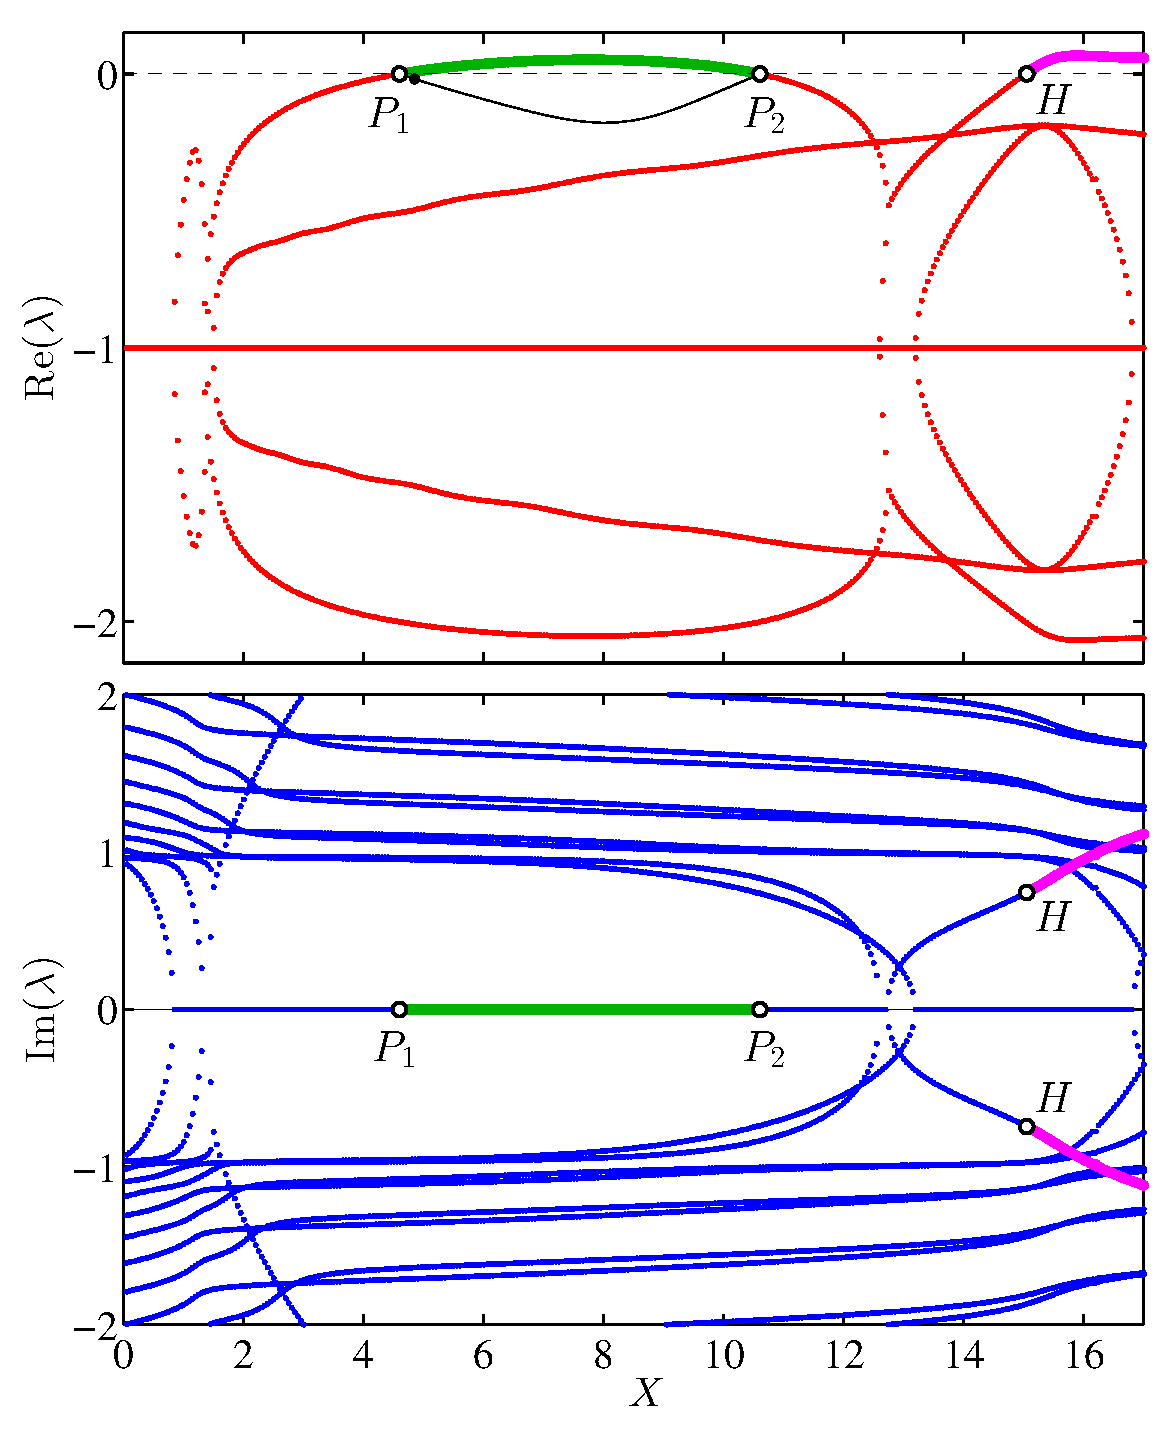
\includegraphics[width=0.9\textwidth]{frequencySpectrumNN.eps}}
  \rule{35em}{0.5pt}
\caption[LL Equation Linearization Spectrum for the Symmetric and Asymmetric 
Steady State Solutions]{Linearization spectrum for the symmetric and asymmetric 
steady state solutions of 
the Lugiato-Lefever equation (\ref{LugiatoLefever})
as the pump power $X$ is varied for $\Delta = 0.92$ and $T_0=2.3$.  
The top and bottom panels depict, respectively, the real and imaginary
parts of the eigenvalues.
%
Stable symmetric solutions bearing Re$(\lambda)<0$ are depicted by 
small (red) dots in the top panel while unstable symmetric solutions 
are depicted with thick solid lines.
%
The thick (green) solid line between the points $P_1$ and $P_2$ represents
the unstable solutions through a forward ($P_1$) and reverse ($P_2$)
pitchfork bifurcations.
%
The thin (black) curve between the points $P_1$ and $P_2$ corresponds to the 
stable asymmetric solution branches created through the pitchfork bifurcation.
(The small black dot next to the point $P_1$ is the stable eigenvalue
used for the slope computation in Fig.~\ref{PitchPhasePortrait}.)
%
The thick (magenta) solid line to the right of the Hopf bifurcation point
$H$ indicates the onset of instability for the symmetric state and the 
existence of an asymmetric periodic solution.
%
}
\label{fig:frequencySpectrum}
\end{figure}
%%%%%%%%%% Fig 1 %%%%%%%%%%%%%%%%%%%%%%%%%%%%%%%%%


Figure~\ref{fig:frequencySpectrum} depicts the linearization 
spectrum for the symmetric stationary
solution [see (red) dashed line in panels (c) and (d) of Fig.~\ref{fig:evolution}] 
as a function of the pump peak power.  
%
The spectrum in Fig.~\ref{fig:frequencySpectrum} evidences the existence of two 
unstable branches:
%
(i) a pitchfork bifurcation loop containing a forward pitchfork 
bifurcation, see point $P_1$ at $X\approx 4.6$, and a reverse pitchfork
bifurcation, see point $P_2$ at $X\approx 10.6$, and 
%
(ii) a Hopf bifurcation, see point $H$ at $X\approx 15.1$.
%
The pitchfork bifurcation, see thick (green) line between the 
points $P_1$ and $P_2$ in Fig.~\ref{fig:frequencySpectrum}, 
is responsible, as the pump power is increased, for the loss of stability of the 
symmetric state towards a pair of asymmetric states (one to the left and one to the 
right) at $P_1$. As the pump power is increased, a reverse pitchfork at $P_2$
is responsible for the collision (and annihilation) of the two asymmetric states 
towards the symmetric state that recovers its stability.
%
A sample of the dynamic destabilization of the (unstable) symmetric state
for a pump strength $X=8$, namely between the two pitchfork points, is depicted 
in Fig.~\ref{fig:evolution}(a). As the figure shows, the symmetric state 
[see dashed (red) line in Fig.~\ref{fig:evolution}(c)] destabilizes
towards the stable, asymmetric state [see solid (blue) line in
Fig.~\ref{fig:evolution}(c)].
%
On the other hand, the instability due to the Hopf bifurcation branch,
see the thick (magenta) line emanating from the point $H$ in
Fig.~\ref{fig:frequencySpectrum}, is responsible for the instability of
the symmetric state towards a {\em periodic} (in $z$) solution. A sample of the
evolution for the symmetric state towards the stable periodic solution
is depicted in Fig.~\ref{fig:evolution}(b). The periodic solution contains
three ``humps'' in its $\tau$ dependence: 
a central one performing left-to-right oscillations while
the side ``humps'' oscillate alternatively up-and-down. Snapshots for the
asymmetric states when the side ``humps'' have the largest magnitude are
depicted in panel (d) corresponding to the times depicted by horizontal
white lines in panel (b).

%%%%%%%%%% Fig 2 %%%%%%%%%%%%%%%%%%%%%%%%%%%%%%%%%%%%%%%%%%%%%%%%
\begin{figure}[t]
\centering
\centerline{
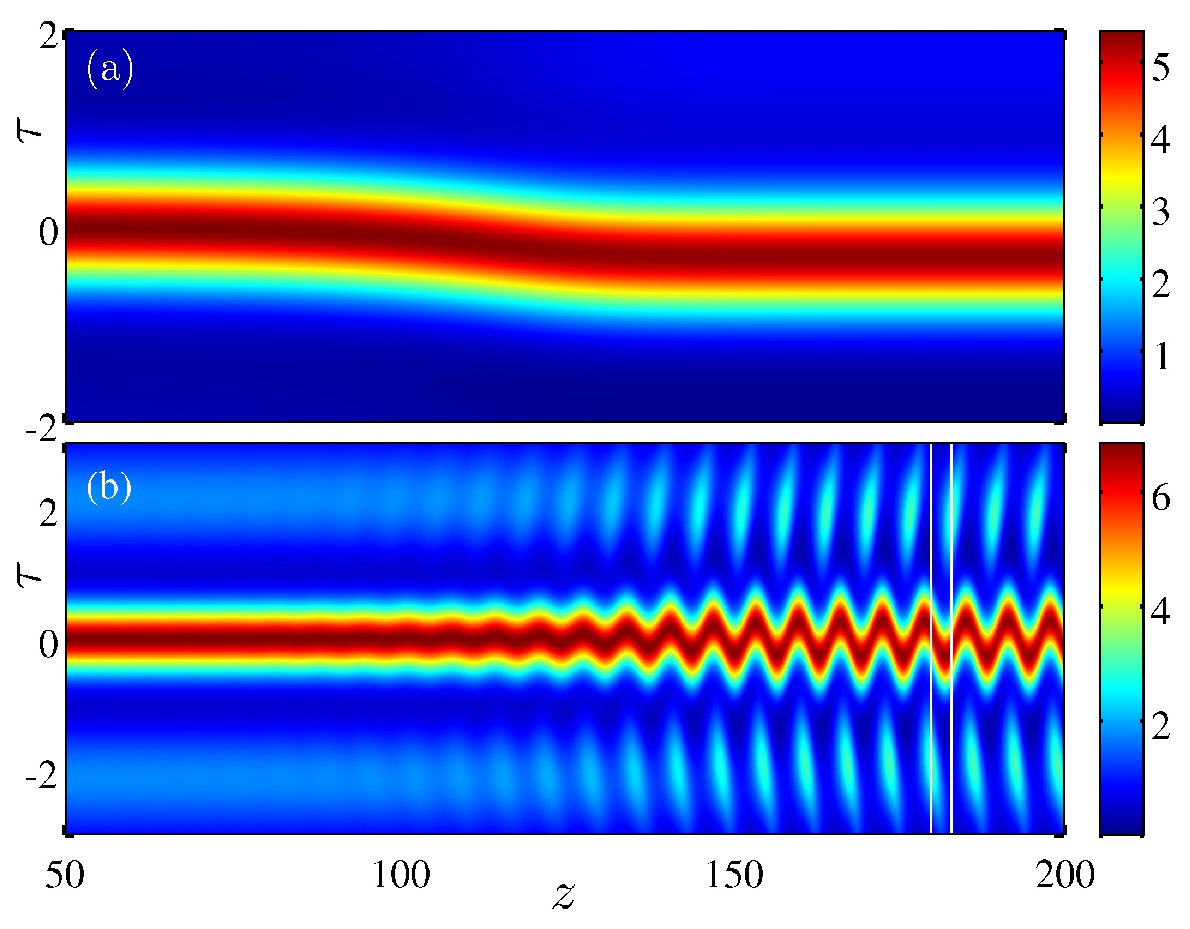
\includegraphics[width=0.85\textwidth]{densityX8X16_t.eps}}
\centerline{ 
\includegraphics[width=0.85\textwidth]{snaps_X8_X16.eps}
\vspace{-0.3cm}
}
  \rule{35em}{0.5pt}
\caption[Density Evolution of Unstable Symmetric States at $X=8$ and 16 and Snapshots]{
(a), (b) Examples for the density evolution of unstable symmetric states
and 
(c), (d) snapshots for the corresponding states.
%
(a) Evolution of unstable symmetric state for $X=8$ between the two pitchfork bifurcations 
$P_1$ and $P_2$ depicted in Fig.~\ref{fig:frequencySpectrum}. The initial symmetric state,
see dashed (red) line in panel (c) evolves towards the asymmetric steady state
depicted in solid (blue) in panel (c).
%
(b) Evolution of unstable symmetric state towards a periodic breathing solution
for $X=16$ (i.e., to the right of the Hopf bifurcation point $H$ in 
Fig.~\ref{fig:frequencySpectrum}). The initial symmetric state [dashed (red)
line] and two snapshots of the density for the periodic solution [solid (blue and 
light blue) lines] separated by half a period, at the times corresponding to the white
vertical lines in panel (b), are depicted in panel (d).
\label{fig:evolution}}
\end{figure}
%%%%%%%%%% Fig 2 %%%%%%%%%%%%%%%%%%%%%%%%%%%%%%%%%%%%%%%%%%%%%%%%

It is important to mention that, due to the cavity loss term ($-iu$), the
real part of the spectrum is symmetric with respect to Re$(\lambda)=-1$
(see Sec.~\ref{secGalerkin} for details).
Therefore, tuning the cavity loss parameter is crucial to the existence of the
SSB bifurcation as higher values of this parameter shift the real part of the
spectrum down precluding the possibility of eigenvalues crossing the
origin and leading to such bifurcations. By the same token, reducing the value
of the cavity loss parameter will induce more eigenvalues to cross the
origin and thus lead to richer and more complicated bifurcation scenarios.
A detailed analysis of the bifurcations as the cavity loss parameter is
varied is outside of the scope of the present dissertation work and will be
studied in a future work.

\clearpage
\JMR{\subsection{Numerical Convergence of the Stability Spectrum}}
\label{secEigs}
\JMR{The purpose of this subsection is to briefly discuss the numerics used for analyzing the frequency spectrum (see Fig.~\ref{fig:frequencySpectrum}) which are dependent on the discretization of fast-time $h = d\tau$, the domain length $L$, and the boundary condition.  The eigenvalue problem Eq.~(\ref{PDEEigenProblem}) can be recast as $i\lambda \vec{\xi}  = M \vec{\xi}$.  This is numerically solved using second-order central differencing in one dimension for the Laplacian given by 
\begin{align}
\nabla^2 u_j = \frac{\partial^2 u}{\partial \tau^2}\bigg|_j \approx \frac{u_{j+1} - 2u_j + u_{j-1}}{h^2},
\end{align}
%
and when implemented into the $M_1$ matrix, yields a matrix $A$ which is tridiagonal except from the matrix elements corresponding to the boundary conditions.  Since boundary conditions of the fast-time differencing in a PDE like the LL model have the potential to alter the stability, it is necessary to compare the stability for each of the specific boundary conditions we would like to use.  For this discussion we limit ourselves to three boundary conditions~\cite{LeVeque}:  Dirichlet, Neumann, and periodic.}

\JMR{In our analysis, we consider a uniform grid with spacing $h$ on the interval $[-L/2, L/2]$.  Dirichlet boundary conditions specify a fixed constant value along the boundary of the domain.  For our Dirichlet boundary conditions we define $u(-L/2) = u(L/2) = 0$ given that the solution has the form of a bright soliton.  Using such a formulation the Laplacian matrix with these Dirichlet boundary conditions becomes
\begin{align}
A  = \frac{1}{h^2} \begin{bmatrix} -2 & 1 &  0  &  \cdots  & 0 \\ 1 & -2 & 1  &  \cdots & 0 \\
0 & \ddots & \ddots & \ddots &  0 \\
0 & 0 & 1& -2 & 1 \\
0 & \cdots & 0 & 1 & -2
  \end{bmatrix}.
\end{align} 
%
Neumann boundary conditions specify the value of the derivative of a solution at the boundary of the domain.  We use a no flux boundary in which $\partial_\tau u(-L/2)= \partial_\tau u(L/2) =0$ such that the Laplacian matrix becomes
\begin{align}
A  = \frac{1}{h^2} \begin{bmatrix} -2 & 2 &  0  &  \cdots  & 0 \\ 1 & -2 & 1  &  \cdots & 0 \\
0 & \ddots & \ddots & \ddots &  0 \\
0 & 0 & 1& -2 & 1 \\
0 & \cdots & 0 & 2 & -2
  \end{bmatrix}.
\end{align}
%
The periodic boundary condition is defined as $u(-L/2) = u(L/2)$ and is justified in the scenario of a ring cavity.  The discretized Laplacian matrix for periodic boundary conditions is
\begin{align}
A  = \frac{1}{h^2} \begin{bmatrix} -2 & 1 &  0  &  \cdots  & 1 \\ 1 & -2 & 1  &  \cdots & 0 \\
0 & \ddots & \ddots & \ddots &  0 \\
0 & 0 & 1& -2 & 1 \\
1 & \cdots & 0 & 1 & -2
  \end{bmatrix}.
\end{align}}
%
\JMR{In order to quantify the convergence of the eigenvalues for $h=0.01$, 0.05, 0.1 and 0.5 given $L=10$, 20, 50, 100, and 200 we analyze the spectrum and the Euclidean norm of matrix $M$ for the symmetric state at $X=8$ which is unstable.  If we consider the 2-norm, then we can show the  convergence by explicitly computing the eigenvectors and eigenvalues of the matrix $M$ in Eq.~(\ref{PDEEigenProblem}) [$i\lambda \vec{\xi}  = M \vec{\xi}$].  Since the matrix $M$ from Eq.~(\ref{PDEEigenProblem}) is symmetric, the 2-norm of $M$ is equal to its spectral radius ($\rho(M)$):
\begin{align}
\lvert \lvert M\lvert \lvert_2 = \rho(M) = \max_{1 \le p \le N} \lvert \lambda_p \lvert,
\end{align} 
where $\lambda_p$ is the $p$th eigenvalue of the matrix~\cite{LeVeque}.  Therefore, we will use the spectral radius to give insight into the convergence between the different boundary conditions.  Table~\ref{dxsmall} compares the spectral radius with various domain lengths $L$ and discretization $h$ for the Dirichlet, Neumann, and periodic boundary conditions.  From Table~\ref{dxsmall} we find a small spectral radius for $h=0.5$ ($\rho(M) \approx 17$) when compared to the $h=0.01$ ($\rho(M) \approx 1,600$), which gives an upper bound to the spectral radius.  Therefore, $h=0.5$ is too coarse a grid size with a small spectral radius which does not accurately capture the true eigenvalues.  %Table~\ref{dxsmall} depicts spectral radius of all three boundary conditions for domain lengths greater than $L=10$.  
The spectral radius alone does not explicitly define if the solutions converge to the true eigenvalues.  Therefore, we will also compare the unstable eigenvalue for this system as a measure of convergence between the different boundary conditions.  Table~\ref{unstableeigTable} compares the unstable eigenvalue for various domain lengths $L$ and discretization $h$ for Dirichlet, Neumann, and periodic boundary conditions.  We omit $h=0.5$ since this discretization is too coarse and does not converge to a single unstable eigenvalue for all boundary conditions.  From Table~\ref{unstableeigTable}, we find the largest descretization for convergence of the unstable eigenvalue is $h=0.1$. }

\JMR{\begin{table}[htb!]
\centering
\ra{1.3}
\begin{tabular}{@{}lllllll@{}}\toprule
&& \multicolumn{5}{c}{Domain Length $L$}  \\
\cmidrule{3-7}
&& $10$ & $20$ & $50$ & $100$ & $200$ \\ \midrule
$h = 0.01$ && $N= 1001$ & $N = 2001$ & & & \\ %$N = 5001$ &  & \\ %$N = 10000$ & $N = 20000$ \\
Dirichlet &&    1.6003$\times10^3$ &  1.6008$\times10^3$ & & & \\ 
Neumann && 1.6003$\times10^3$ & 1.6008$\times10^3$ & & & \\ 
Periodic && 1.6007$\times10^3$ & 1.6009$\times10^3$ & & & \\ \midrule
$h = 0.05$ && $N= 201$ & $N = 401$ & $N = 1401$ & $N = 2001$ & \\ % $N = 4001$ \\
Dirichlet && 1.6003$\times10^3$ &1.6008$\times10^3$ & 1.6009$\times10^3$ & 1.6009$\times10^3$ & \\ 
Neumann && 1.6135$\times10^3$ & 1.6136$\times10^3$ & 1.6136$\times10^3$ &1.6136$\times10^3$ & \\ 
Periodic && 1.6007$\times10^3$ & 1.6009$\times10^3$ & 1.6009$\times10^3$ & 1.6009$\times10^3$ & \\ \midrule
$h = 0.1$ && $N= 101$ & $N = 201$ & $N = 501$ & $N = 1001$ & $N = 2001$ \\
Dirichlet && 400.2982 &400.7857  & 400.9032 & 400.9170 & 400.9202 \\ 
Neumann && 404.0546 & 404.0741 & 404.0741 & 404.0741& 404.0741 \\ 
Periodic &&  400.7203 & 400.8860 & 400.9167 & 400.9202 & 400.9210 \\  \midrule
$h = 0.5$ && $N= 21$ & $N = 41$ & $N = 101$ & $N = 201$ & $N = 401$ \\
Dirichlet &&  16.4045 & 16.8224 &  16.9319 & 16.9454 & 16.9485\\ 
Neumann && 16.9710 & 17.0662 & 17.0682 & 17.0682 & 17.0682 \\ 
Periodic && 16.7560 & 16.9149 & 16.9450 & 16.9485 & 16.9493\\ 
\bottomrule
\end{tabular}
\caption[Comparison of the Spectral Radius for Dirichlet, Neumann, and Periodic Boundary Conditions]{Comparison of the spectral radius for Dirichlet, Neumann, and periodic boundary conditions. For discretization size $h = 0.01$, we used two domain lengths $L = 10$ and 20 corresponding to Laplacian matrix size of $N\times N$ .  Given $h=0.5$ four domain lengths $L = 10$, 20, 50, and 100 are compared between the three boundary conditions.  For $h=0.1$ and 0.5 five domain lengths $L = 10$, 20, 50, 100 and 200 are compared.  The spectral radius for $h=0.5$ is too coarse a discretization and fails to converge to the proper eigenvalues.}%The spectral radius for $h=0.5$ does not converge.}
\label{dxsmall}
\end{table}}

\begin{landscape}
\begin{table}[htb!] 
\centering
\ra{1.3}
\begin{tabular}{@{}lllllll@{}}\toprule
&& \multicolumn{5}{c}{Domain Length $L$}  \\
\cmidrule{3-7}
&& $10$ & $20$ & $50$ & $100$ & $200$ \\ \midrule
$h = 0.01$ && $N= 1001$ & $N = 2001$ & & & \\ %$N = 5001$ &  & \\ %$N = 10000$ & $N = 20000$ \\
Dirichlet && 0.052680703192848 & 0.051828350475447 & & & \\ 
Neumann && 0.053646211533514 &  0.051828322918270 & & & \\ 
Periodic && 0.052679254860875 & 0.051828350684082 & & & \\ \midrule
$h = 0.05$ && $N= 201$ & $N = 401$ & $N = 1401$ & $N = 2001$ & \\ % $N = 4001$ \\
Dirichlet && 0.052671286287013 & 0.051840500243317 & 0.051840521421259 & 0.051840521421264 & \\ 
Neumann && 0.053622508462011 & 0.051840474228158 & 0.051840521421259 & 0.051840521421258 &\\ 
Periodic && 0.052663061760651 & 0.051840501211644 & 0.051840521421264 & 0.051840521421259 & \\ \midrule
$h = 0.1$ && $N= 101$ & $N = 201$ & $N = 501$ & $N = 1001$ & $N = 2001$ \\
Dirichlet && 0.052689738246259 & 0.051881121063754 & 0.051881142017631 & 0.051881142017632 & 0.051881142017631 \\ 
Neumann && 0.053620924363313 &  0.051881096702647 &  0.051881142017629 & 0.051881142017633 & 0.051881142017632 \\ 
Periodic && 0.052671246337099 & 0.051881122829374 & 0.051881142017631 & 0.051881142017631 & 0.051881142017633\\  \midrule
\bottomrule
\end{tabular}
\caption[Comparison of Unstable Eigenvalue for Dirichlet, Neumann, and Periodic Boundary Conditions]{Comparison of unstable eigenvalue for Dirichlet, Neumann, and periodic boundary conditions.  The layout is the same as Table~\ref{dxsmall}.  The discretization $h=0.5$ is omitted because it fails to converge to a single unstable eigenvalue.  The largest discretization to use for convergence is $h=0.1$.}
\label{unstableeigTable}
\end{table}
\end{landscape}

\JMR{\begin{figure}[htb!]
\centering
\centerline{
\begin{subfigure}{0.5\textwidth}
\hspace{0.5cm}\includegraphics[width=0.9\linewidth]{EigPlot_1.eps}
\caption{$h = 0.01$ }
\end{subfigure}
\begin{subfigure}{0.5\textwidth}
\hspace{0.5cm}\includegraphics[width=0.9\linewidth]{EigPlot_3.eps}
\caption{$h = 0.05$ }
\end{subfigure}}
\centerline{
\begin{subfigure}{0.5\textwidth}
\hspace{0.5cm}\includegraphics[width=0.9\linewidth]{EigPlot_7.eps}
\caption{$h = 0.1$ }
\end{subfigure}
\begin{subfigure}{0.5\textwidth}
\hspace{0.5cm}\includegraphics[width=0.9\linewidth]{EigPlot_12.eps}
\caption{$h = 0.5$ }
\end{subfigure}}
  \rule{35em}{0.5pt}
\caption[Comparison of Frequency Spectrum for Domain Length $L$=10]{Comparison of the frequency spectrum for the domain length $L=10$ for (a) $h=0.01$, (b) $h=0.05$, (c) $h=0.1$, and (d) $h=0.5$.  Each plot depicts the frequency spectrums for Dirchlet (green), Neumann (red), and periodic (blue) boundary conditions.  The discretization (d) $h=0.5$ is too coarse and does not converge. }
\label{figAdd1}
\end{figure}
}

\JMR{\begin{figure}[htb!]
\centering
\centerline{
\begin{subfigure}{0.5\textwidth}
\hspace{0.5cm}\includegraphics[width=0.9\linewidth]{EigPlot_5.eps}
\caption{$h = 0.05$ }
\end{subfigure}
\begin{subfigure}{0.5\textwidth}
\hspace{0.5cm}\includegraphics[width=0.9\linewidth]{EigPlot_9.eps}
\caption{$h = 0.1$ }
\end{subfigure}}
\centerline{
\begin{subfigure}{0.5\textwidth}
\hspace{0.5cm}\includegraphics[width=0.9\linewidth]{EigPlot_14.eps}
\caption{$h = 0.5$ }
\end{subfigure}}
  \rule{35em}{0.5pt}
\caption[Comparison of Frequency Spectrum for Domain Length $L=50$]{Comparison of the frequency spectrum for the domain length $L=50$ for (a) $h=0.05$, (b) $h=0.1$, and (c) $h=0.5$.  Each plot has same layout as Fig.~\ref{figAdd1}.  The domain length $L=50$ is adequately contains the steady state solution without truncation; therefore, the solution tends to zero at the boundary.  The three boundary conditions [Dirichlet (green), Neumann (red), and periodic (blue)] converge for $h=0.1$ and $h=0.05$.  The discretization (c) $h=0.5$ is too coarse and does not converge.}
\label{figAdd2}
\end{figure}
}

\JMR{Figure~\ref{figAdd1} compares the frequency spectrum for the three boundary conditions using a domain length $L = 10$ for various discretization [(a) $h = 0.01$, (b) $h= 0.05$, (c) $h=0.1$ and (d) $h = 0.5$ (which truncates the solution)].  In Fig.~\ref{figAdd1}, the Neumann (red) and periodic (blue) boundary conditions are comparable; however the Dirichlet (green) boundary conditions have discrepancies due to imposing an invalid criteria that the solution is zero at the boundary.  %There are discrepancies between a few eigenvalues using the Dirichlet boundary condition due to forcing zero solutions at the boundaries of the domain.  
For domain length $L=10$, the steady state solution is truncated and is not zero along the boundary.  A more accurate choice of Dirichlet boundary condition would be $u(-L/2) = \alpha$ and $u(L/2) = \beta$ where $\alpha$ and $\beta$ are constants.  Figure~\ref{figAdd2} compares the domain length $L=50$ for various discretization [(a) $h = 0.05$, (b) $h=0.1$, and (c) $h=0.5$] for the three boundary conditions.  The larger domain length depicts agreement between all three boundary conditions except for large $h$=0.5 (in agreement with Table~\ref{dxsmall}).  Both Figs.~\ref{figAdd1}(d) and~\ref{figAdd2}(c) show no convergence for $h=0.5$, which is too coarse a step size for use in the LL model.  The numerical discretization, domain length and boundary conditions can influence the stability analysis.  Based on Tables~\ref{dxsmall} and \ref{unstableeigTable}, we can conclude a maximum discretization $h=0.1$ to use for convergence.  As the domain length is increased the convergence also improves but at the cost of a larger matrix size.  For $L\ge 20$ and $h\le 0.1$, the three boundary conditions are in good agreement and converge to the same frequency spectrum.  Based on these results, for the spectrum in Fig.~\ref{fig:frequencySpectrum} we used the Dirichlet boundary condition, domain length $L = 50$ and discretization $h$ = 0.1, which converge to the frequency spectrum for the eigenvalue problem Eq.~(\ref{PDEEigenProblem}).}


%%%%%%%%%% Section Numerical Results
\subsection{Bifurcation Analysis Using the NCVA Approach
\label{secNCVA:app}}
%
We apply the NCVA to Eq.~(\ref{LugiatoLefever}) to verify if the reduced
dynamical system is able to qualitatively (and quantitatively) capture the 
SSB instability by following all temporally symmetric and asymmetric solutions 
to the reduced system of ODEs given by %Eq.~(\ref{NCVAODE}).
%Then, the modified Euler-Lagrange equations for the effective Lagrangian $L = \int_{-\infty}^\infty \mathcal{L}_T d\tau$ yield
%%
\begin{equation}
%\frac{\partial p}{\partial t} = \frac{\partial \mathcal{L}}{\partial u} \equiv \frac{\partial L}{\partial u} + \left[ \frac{\partial R}{\partial u_- }\right]_{\mathrm{PL}}.
\frac{\partial L}{\partial u} - \frac{d}{dt}\left( \frac{\partial L}{\partial \dot{u}} \right) + \int_{-\infty}^\infty \left[ \frac{\partial \mathcal{R}}{\partial u_- }\right]_{\mathrm{PL}} d\tau = 0. 
\label{NCVAODE}
\end{equation}
%
The conservative Lagrangian density for the NLS, namely Eq.~(\ref{LugiatoLefever})
with the right-hand-side equal to zero, is
%
\begin{equation}
\mathcal{L} = \frac{i}{2} \left(u^* u_z- u u_z^*\right) -  \left\vert u_{\tau}\right\vert^2 +  \frac{1}{2}\left\vert u \right\vert^4 - \Delta \left\vert u \right\vert^2.
\end{equation}
%
Here, we construct $\left[ \partial \mathcal{R}/\partial u_- \right]_{\mathrm{PL}} = - iu + i S(\tau)$, by choosing $\mathcal{R} = \left( -iu_{+} + i S(\tau) \right)u_-$.  Therefore, the relevant non-conservative Lagrangian density can be written as
%
\begin{eqnarray}
\mathcal{L} &=& \frac{i}{2} \left(u_{1}^* u_{1,z}- u_{1} u_{1,z}^*\right) -  \left\vert u_{1,\tau}\right\vert^2 + \frac{1}{2} \left\vert u_1 \right\vert^4 -  \Delta  \left\vert u_1 \right\vert^2  \nonumber
 \\
&-& \frac{i}{2} \left(u_{2}^* u_{2,z}- u_{2} u_{2,z}^*\right) +  \left\vert u_{2,\tau}\right\vert^2 -\frac{1}{2}  \left\vert u_2 \right\vert^4 +  \Delta  \left\vert u_2 \right\vert^2  \nonumber \\ 
&+& \left( - iu_{+} + i S(\tau) \right)u_-,  
\end{eqnarray}
%
where $u_1 = \left( 2u_+ + u_- \right)/2$ and $u_2 = \left(2u_+ - u_- \right)/2$.
%
For reasons of brevity, we chose to express the Lagrangian density above
in 1,2 coordinates. Writing the Lagrangian in $\pm$ coordinates lends
itself to lengthier expressions but to more straightforward implementation
of the physical limit where the (+) variables directly coincide with the
physical variables [and the $(-)$ variables are eliminated].
%
From $\mathcal{L} $, we can derive, through the Euler-Lagrange
equations (\ref{NCVAODE}), the full LL model at the PDE level.
In order to, however, obtain an analytical insight in the dynamics
of the model, our aim is to use an ansatz approximation of the
pulse reducing its Lagrangian to a Lagrangian over effective
(yet time-dependent) properties of its form, like the amplitude,
the width and its center of mass, among others. Then for these
effective properties, in the spirit of Refs.~\cite{JuliaNCVA,ref4},
a coupled system of 
ODEs approximating
the dynamical evolution will be derived and, perhaps more
importantly for our considerations, their corresponding steady
states and possible bifurcations will be amenable to 
analysis. 

Applying the NCVA methodology described above to the LL model
(\ref{LugiatoLefever}) where \begin{align}
\left[ \frac{\partial \mathcal{R}}{\partial
u_- }\right]_{\mathrm{PL}} = -iu  + i S(\tau), \end{align}
 yields 
\begin{align}
\mathcal{R} = \left( -iu_{+}  + i S(\tau) \right)u_-.
\end{align}  
%
We first choose the following simple Gaussian ansatz
%
\begin{equation}
\bar{u}_j = a_j \exp\left[-\frac{(\tau-\xi_j)^2}{2\sigma_j^2}\right] \exp(i\,b_j),
\quad j=1,2
\label{eq:4pAnsatz}
\end{equation}
%
where height $a$, center position $\xi$, width $\sigma$, and phase $b$ 
are the variational parameters.  
%
The ansatz was selected as the simplest localized waveform with freedom
to move left or right in order to capture, in the simplest sense,
a possible asymmetry in the solution of the original LL model.
%
Applying the NCVA method with this, arguably 
over-simplified, four-parameter ansatz, 
leads, through the Euler-Lagrange equations, to a system of algebraic 
differential equations for which the derivatives of the variational
parameters cannot be solved for explicitly. Nonetheless, it is
possible to obtain algebraic equations for the corresponding 
steady state ($\dot{a} = \dot{b} = \dot{\xi} = \dot{\sigma} = 0$)
solutions of the form:
%
\begin{align}
%\setlength{\jot}{16pt}
%\begin{cases}
%\frac{a^2\sqrt{\pi}}{2 \sigma^2}+\frac{1}{4} a^4\sqrt{2 \pi}+\Delta a^2\sqrt{\pi} &= \frac{2a\sqrt{X}\sin(b)\sqrt{2\pi}T_0^3}
%{(T_0^2+2\sigma^2)^{3/2}}, \\[1em] \nonumber
%2a^2\sigma\sqrt{\pi} &= \frac{2 \sqrt{X}a\cos(b)\sqrt{2\pi}\sigma T_0}{\sqrt{T_0^2+2\sigma^2}}, \\[1em] \nonumber
%-\frac{a\sqrt{\pi}}{\sigma}+a^3\sqrt{2\pi}\sigma+2\Delta a\sigma\sqrt{\pi} &= \frac{2\sqrt{X}\sin(b)\sqrt{2\pi}\sigma T_0}
%{\sqrt{T_0^2+2\sigma^2}}, \\[1em] \nonumber
%0 &= \frac{-2\sqrt{X}a\xi\sin(b)\sqrt{2\pi}T_0}{\sigma\sqrt{T_0^2+2\sigma^2}}. \\
%\end{cases}
%\end{align}
\begin{cases}
\frac{a^2\sqrt{\pi}}{2 \sigma^2}+\frac{1}{4} a^4\sqrt{2 \pi}+\Delta a^2\sqrt{\pi} &= \frac{a\sin(b)T_0^2 \beta}
{(T_0^2+2\sigma^2)}, \\[1em]
2a^2\sigma\sqrt{\pi} &=  a \cos(b) \sigma \beta, \\[1em]
-\frac{a\sqrt{\pi}}{\sigma}+a^3\sqrt{2\pi}\sigma+2\Delta a\sigma\sqrt{\pi} &= \sin(b) \sigma \beta, \\[1em]
0 &= \frac{-a\xi\sin(b)\beta}{\sigma},
\end{cases}
\label{4pE}
\end{align}
%
where $\beta = \frac{2\sqrt{2 \pi X} T_0}{\sqrt{T_0^2 + 2 \sigma^2}}$.  


Figure~\ref{figSSB4p} depicts the comparison of the bifurcation diagrams
for steady state solutions obtained from the original LL 
model~(\ref{LugiatoLefever}) and the NCVA approach for $\Delta =0.92$ 
and $T_0=2.3$ by monitoring $|u (\tau=0)|^2$ as a function of pump 
peak power $X$, in line with the earlier work of Ref.~\cite{XuCoen}.
%
Both solutions for the original LL model and the algebraic NCVA system
are obtained by numerical continuation using a standard fixed point iteration 
(Newton-Krylov).
%
The solutions for the LL model are depicted by the thick curves
while the corresponding NCVA approximations by the thin curves.
Solid and dashed correspond, respectively, to stable and unstable 
solutions.
%
The insets in the figure depict temporal pulse intensity profiles 
$|u|^2$ for $X = 4$ (symmetric), $X=8$ (symmetric and asymmetric), 
and $X=11$ (symmetric) for both the LL model (thick curves)
and the NCVA reconstructions (thin curves).
%
For completeness, the insets also show the corresponding linearization
spectra.
%
As it is evident from the figure, the NCVA with a four-parameter 
ansatz agrees very well with the symmetric branch of LL model
(see black and blue curves). However, for the asymmetric branch
there seems to be a large discrepancy between the LL model and
its NCVA approximation. In fact, as indicated in the figure, the 
asymmetric NCVA branch is unstable while it is stable for the original 
LL model. Upon further inspection (details are omitted for brevity), 
the instability of the asymmetric NCVA branch stems, instead of
a pitchfork bifurcation, from a Hopf bifurcation that creates a stable 
limit cycle in the variational parameters.
%
%%%%%%%%%% Fig 3 %%%%%%%%%%%%%%%%%%%%%%%%%%%%%%%%%%%%%%
\begin{figure*}[t!!]
\centering
\centerline{
\includegraphics[width=0.95\textwidth]{SSBBif4PN.eps}}
  \rule{35em}{0.5pt}
\caption[SSB Bifurcation Diagram Comparison for LL Steady States and NCVA 4-Parameter Ansatz]{Bifurcation for steady states of the LL model (\ref{LugiatoLefever})
(thick curves) and their approximation using the NCVA methodology with the 
over-simplified four-parameter ansatz (\ref{eq:4pAnsatz}) (thin curves)
as the pump strength $X$ is varied for $\Delta = 0.92$ and $T_0 = 2.3$.
%
Stable (Unstable) branches are depicted with solid (dashed) lines.
%
The (red and green) branches bifurcating from the main branch (blue and 
black lines) correspond to asymmetric solutions.
%
The insets depict the pulse temporal intensity profiles obtained for 
$X=4, 8$ (symmetric and asymmetric), and $X=11$ (symmetric) for
the original LL model (thick curves) and their NCVA approximation
(thin curves).
%
The insets also depict the corresponding stability spectra
for these solutions where stable eigenvalues are depicted in blue 
and unstable eigenvalues in red.
\label{figSSB4p}}
\end{figure*}
%%%%%%%%%% Fig 3 %%%%%%%%%%%%%%%%%%%%%%%%%%%%%%%%%%%%%%

It is evident that the four-parameter ansatz is unable to predict the
existence of the pitchfork loop of the original LL model and, furthermore,
although it is able to predict a SSB bifurcation, it fails to give an 
accurate estimation for its threshold (i.e., the critical
pump power needed to observe asymmetric states).
%
However, this over-simplified ansatz gives two valuable insights regarding 
how to make a more judicious choice for our ansatz. 
%
Firstly, the ansatz~(\ref{eq:4pAnsatz}) has an inherent complication in that
its corresponding Euler-Lagrange equations lead to a degenerate system
of differential-algebraic equations which can only be explicitly written
for the steady state. 
%
This degeneracy can be circumvented, as we will show below, by proper balancing 
of the variational parameters in an ansatz with more degrees of freedom.
%
Secondly, and more importantly, the four-parameter ansatz, by construction, 
only corresponds to real solutions (up to a global phase shift) that lack a 
$\tau$-dependence on their phase.
%
This lack of $\tau$-dependence on the phase is responsible for the
ansatz solution's lack of internal flow of the field $u$
along the $\tau$-direction.  To showcase the importance of a nontrivial $\tau$-dependence on the phase, on may transform the NLS equation through the Madelung transformation $u=\sqrt{\rho}\,e^{i\phi}$ such that the wavefunction is recast in terms of its density $\rho$ and phase $\phi$.  Through the Madelung transform, we can obtain an evolution equation for the density that corresponds to an inviscid Eulerian fluid with the fluid velocity $v$ given precisely by $v = \nabla \phi$.  Thus, the fluid velocity for the system can be obtained by computing
the gradient of the phase of the solution at hand.
Therefore, a lack of a phase variation in the solution
implies a lack of internal fluid flow for the solution. 
%
%\footnote{We remind the reader that when transforming the
%NLS equation through the Madelung transformation
%$u=\sqrt{\rho}\,e^{i\phi}$ (i.e., writing the wavefunction in
%terms of its density $\rho$ and phase $\phi$), one obtains
%an evolution equation for the density that corresponds to
%an inviscid Eulerian fluid (incorporating the so-called
%quantum pressure term that is not important for the current
%argument) with the fluid velocity $v$ given precisely by $v=\nabla \phi$.
%Thus, the fluid velocity for the system can be obtained by computing
%the gradient of the phase of the solution at hand.
%Therefore, a lack of a phase variation in the solution
%implies a lack of internal fluid flow of the solutions.}
%
As we explain below, the asymmetric solution is supported
by a delicate balance of the internal flow within this
steady state solution. 
%albeit the density
%of the solution remaining constant (i.e., it is a steady state
%for the density).
%
The presence of the underlying flow is clear after careful examination
of the (numerically) exact solutions of the original LL model as depicted
in panels (a) and (b) of Fig.~\ref{fig4SSB}. These panels depict the
density (blue) and phase (red) of the solution where the arrows
indicate the regions where the fluid velocity, as defined by the
gradient of the phase, has different directions. 
%
The central density maximum, for both the symmetric and
asymmetric solutions, stems from an inward flow towards the
center [which corresponds to a sink of flow due to high density 
through the loss term $iu$ in Eq.~(\ref{LugiatoLefever})]
while the ``wings'', again for both symmetric and asymmetric solutions, 
are supported by sources of the underlying flow maintained by
the pump.
%
In contrast, the NCVA four-parameter ansatz (\ref{eq:4pAnsatz}) lacks
a phase profile and, therefore, lacks any internal flow as depicted
in panels (c) and (d) of Fig.~\ref{fig4SSB}.
%
It is then clear that the four-parameter ansatz (\ref{eq:4pAnsatz})
should be inadequate for capturing the important effects of
the underlying current flows of the solutions.

%%%%%%%%%% Fig 4 %%%%%%%%%%%%%%%%%%%%%%%%%%%%%%%%%%%%%%%%%%%%%%%%%%%%%%
\begin{figure}[t!]
\centering
\includegraphics[width=0.42\textwidth]{fluidVelocity_X8_pdeSN.eps} \quad
\includegraphics[width=0.42\textwidth]{fluidVelocity_X8_pdeASN.eps}
\\
\includegraphics[width=0.42\textwidth]{fluidVelocity_X8_4PSN.eps} \quad
\includegraphics[width=0.42\textwidth]{fluidVelocity_X8_4PASN.eps}
\\
\centerline{\includegraphics[width=0.42\textwidth]{fluidVelocity_X8_6PSN.eps} \quad
\includegraphics[width=0.42\textwidth]{fluidVelocity_X8_6PASN.eps}}
%\vskip -1.5cm
  \rule{35em}{0.5pt}
\caption[Fluid Velocity of LL Equation and NCVA Solutions]{Understanding the importance of including non-trivial phase
terms in the NCVA ansatz. The different panels depict an overlay of 
(i) the temporal intensity profile of the pump pulse $|S(\tau)|^2$ 
(green dashed line),
(ii) the pulse intensity profile $|u|^2$ (blue), and 
(iii) its corresponding fluid velocity (red, $\times 50$)
for 
(a,b) the LL model (top), 
(c,d) the four-parameter NCVA (middle), and 
(e,f) the six-parameter NCVA (bottom)
for symmetric $X=8$ (left) and asymmetric $X=8$ (right) steady state solutions.
%
The (red) arrows indicate the direction of the fluid velocity which drives 
the SSB bifurcation between the symmetric and asymmetric solutions.
}
\label{fig4SSB}
\vskip -0.5cm
\end{figure}
%%%%%%%%%% Fig 4 %%%%%%%%%%%%%%%%%%%%%%%%%%%%%%%%%%%%%%%%%%%%%%%%%%%%%%


It is important to mention at this stage that steady state solutions
(for the density) in NLS-type settings incorporating loss and gain
terms must necessarily involve underlying flows that carry
``material'' from the gain regions towards the lossy regions.
%
Therefore, in these settings, variational methods should be based
on ans\"atze that incorporate the appropriate underlying current.
%
Inspired by the appreciation of the presence of such underlying flows 
(and their delicate balance in the steady state solutions)
let us choose an ansatz that is capable of supporting such flows.
%
Based on this observation, we introduce a six-parameters ansatz
of the form:
%
\begin{eqnarray}
\bar{u}_j &=&  a_j \exp\left[\frac{-(\tau-\xi_j)^2}{2\sigma_j^2}\right] \;  \exp\left[i(d_j(\tau-\xi_j)^2 + c_j(\tau - \xi_j) + b_j)\right] ,
\label{6pansatz}
\end{eqnarray}
%
where, in addition to the parameters height $a$, center position $\xi$, 
width $\sigma$, phase $b$, we have also introduced  velocity $c$ and 
chirp $d$ as variational parameters.
%
Following again the NCVA methodology for this improved ansatz, we 
obtain the following system of ODEs of the variational parameters:
%
\begin{align}
\begin{cases}
\dot{a} =& \frac{1}{4}\frac{-4a^2\sigma^3\sqrt{\pi}+3\sigma^2I_b-8a^2d\sigma^3\sqrt{\pi}-2I_d}{a\sigma^3\sqrt{\pi}}, \\[1em]
\dot{b} =& -\frac{1}{8}\frac{8a^2\sqrt{\pi}-5a^4\sqrt{2}\sqrt{\pi}\sigma^2-4I_\sigma \sigma^2+6I_a\sigma a-8a^2c^2\sqrt{\pi}\sigma^2}{ a^2\sigma^2\sqrt{\pi}} + \frac{\sigma c I_c-a^2 \Delta\sqrt{\pi}\sigma^2}{a^2\sigma^2\sqrt{\pi}}, \\[1em]
\dot{c} =& -\frac{c I_b+I_{\xi}}{a^2\sigma\sqrt{\pi}}, \\[1em]
\dot{d} =& \frac{1}{4}\frac{4a^2\sqrt{\pi}-16a^2 d^2 \sigma^4\sqrt{\pi}-a^4\sqrt{2}\sqrt{\pi}\sigma^2-4I_s\sigma^2+2I_a\sigma a}
{a^2\sigma^4\sqrt{\pi}}, \\[1em]
\dot{\sigma} =& -\frac{1}{2}\frac{\sigma^2I_b-8a^2 d \sigma^3\sqrt{\pi}-2I_d}{a^2\sigma^2\sqrt{\pi}}, \\[1em]
\dot{\xi} =& \frac{2a^2\sigma c \sqrt{\pi}+I_c}{a^2\sigma\sqrt{\pi}}, 
\end{cases}
\label{6pE}
\end{align}
%
where the over-dot denotes derivative with respect to $z$.  Although it is possible to explicitly solve for the derivatives
of the variational parameters, the resulting NCVA ODEs are cumbersome
in that they include the terms $I_a, I_b, I_c, I_d, I_{\xi},$ and 
$I_{\sigma}$ which involve integrals that cannot be explicitly evaluated:
%
\begin{align}
\begin{cases}
I_a =& \bigintss\limits_{-\infty}^{\infty} E\sin(\Phi) \,d\tau, \\[0em] \nonumber
I_b =& \bigintss\limits_{-\infty}^{\infty} aE \cos(\Phi) \,d\tau, \\[0em]
\nonumber
I_c =& \bigintss\limits_{-\infty}^{\infty}  a E(\tau-\xi) \cos(\Phi) \,d\tau, \\[1em]
\nonumber
I_d  = &\bigintss\limits_{-\infty}^{\infty} a E(\tau-\xi)^2 \cos(\Phi) \,d\tau ,\\[1em] \nonumber
I_\sigma =&\bigintss\limits_{-\infty}^{\infty} \frac{ a E}{\sigma^3}  \sin(\Phi) \,d\tau,  \\[1em] \nonumber
I_\xi =&\bigintss\limits_{-\infty}^{\infty} \Big[aE \left(-2d(\tau-\xi)-c\right)
\cos(\Phi)  + \frac{ a E(\tau-\xi) }{\sigma^2} \sin(\Phi) \Big] \,d\tau, 
\end{cases}
\end{align}
%
where $\Phi =d(\tau-\xi)^2+c(\tau-\xi)+b$ and $E = 2\sqrt{X}e^{-\frac{ (\tau-\xi)^2}{2 \sigma^2}}e^{-\frac{\tau^2}{T_0^2}} $.
%
Nonetheless, for our numerical studies it suffices to evaluate numerically
these integrals as we seek stationary states or as we follow the
dynamics of the parameters as $z$ changes.

%%%%%%%%%% Fig 5 %%%%%%%%%%%%%%%%%%%%%%%%%%%%%%%%%
\begin{figure}[htb!]
\centering
\centerline{
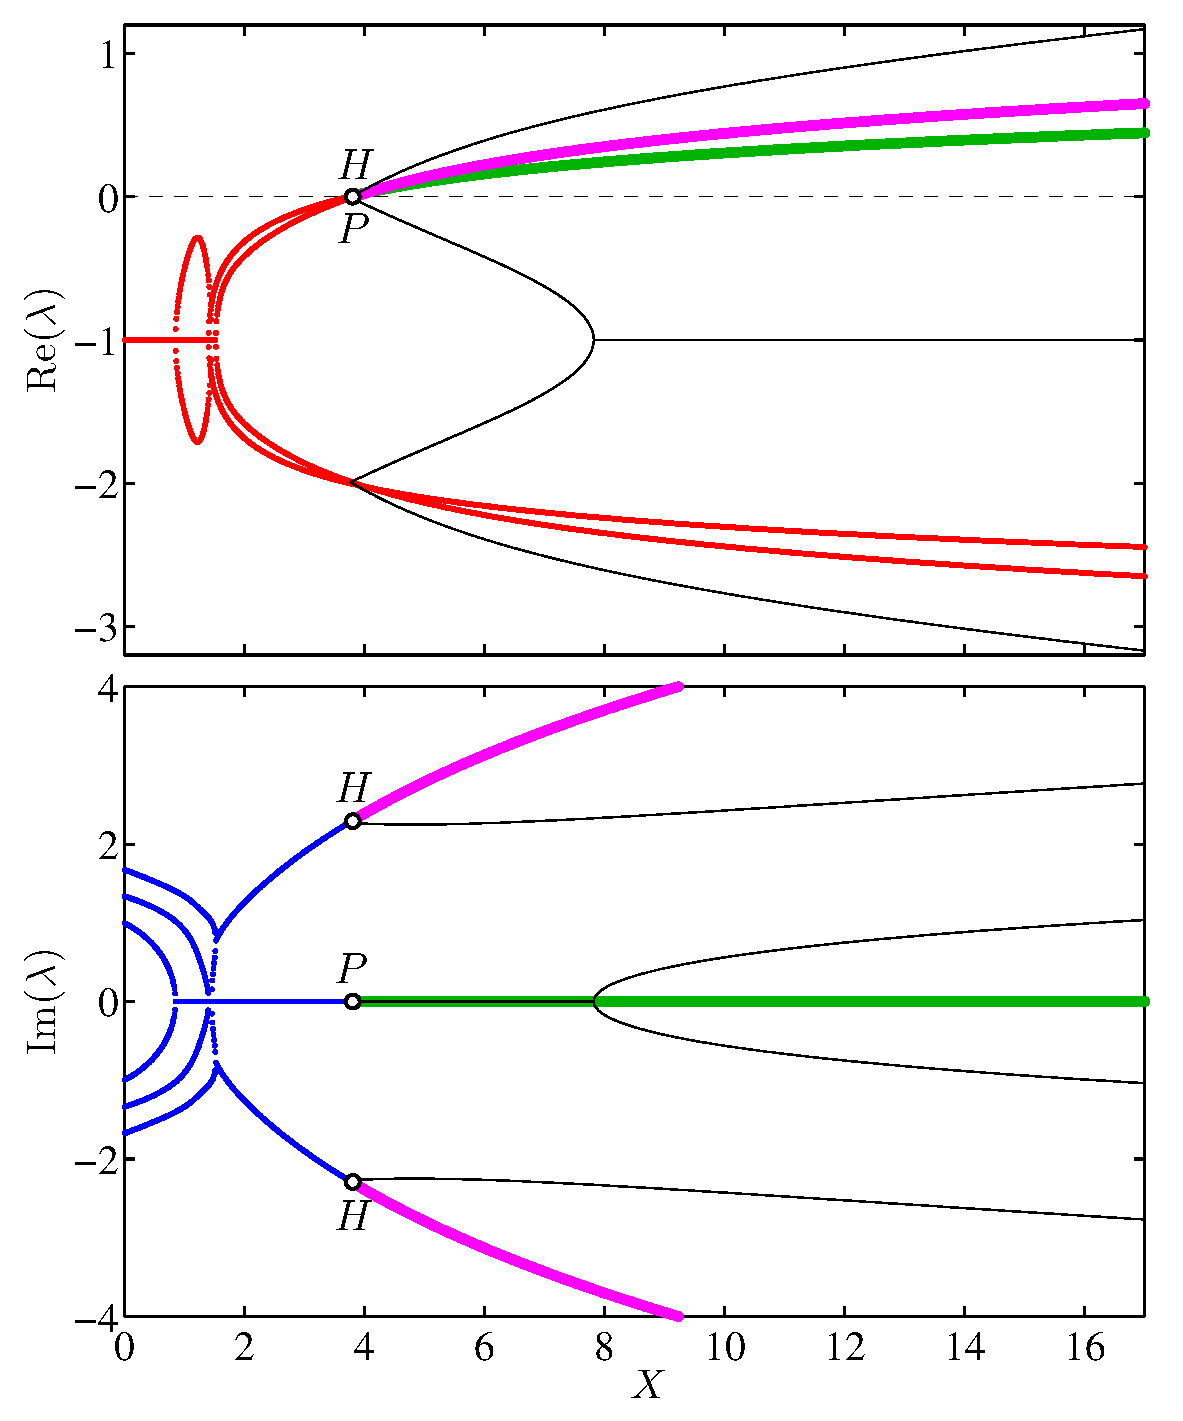
\includegraphics[width=0.9\textwidth]{frequencySpectrum_NCVA.eps}}
  \rule{35em}{0.5pt}
\caption[NCVA ODE Linearization Spectrum]{
Linearization spectrum for the reduced NCVA ODE (\ref{6pE}).
The notation is the same as the spectrum for the original LL model
depicted in Fig.~\ref{fig:frequencySpectrum}.
%
The reduced ODE model displays a degenerate bifurcation
consisting of simultaneous pitchfork (P) and Hopf (H)
bifurcations and thus the asymmetric steady state (see thin black
solid lines) is unstable from its inception.
\label{fig:frequencySpectrum_NCVA}
}
\end{figure}
%%%%%%%%%% Fig 5 %%%%%%%%%%%%%%%%%%%%%%%%%%%%%%%%%

%%%%%%%%%% Fig 6 %%%%%%%%%%%%%%%%%%%%%%%%%%%%%%%%%%%%%%%
\begin{figure*}[htb!]
%\vspace{-0.5cm}
\centering
\centerline{
\includegraphics[width=0.95\textwidth]{SSBBif6PN.eps}}
\caption[SSB Bifurcation Diagram Comparison for LL Steady States and NCVA 6-Parameter Ansatz]{Bifurcation diagram as in Fig.~\ref{figSSB4p} but for the more 
complete six-parameter ansatz (\ref{6pansatz}). Same layout and
meaning as in Fig.~\ref{figSSB4p}.}
\label{figSSB6p}
\end{figure*}
%%%%%%%%%% Fig 6 %%%%%%%%%%%%%%%%%%%%%%%%%%%%%%%%%%%%%%%

Figure \ref{fig:frequencySpectrum_NCVA} depicts the linearization
spectrum for the reduced NCVA six-parameter ODE model (\ref{6pE}) that 
should be compared to the linearization spectrum of original LL model
depicted in Fig.~\ref{fig:frequencySpectrum}.
%
It is clear that both spectra share some of the bifurcation structure 
but, at the same time, they have notable differences.
%
For instance, although the reduced NCVA ODE is able to capture
the SSB at $X\approx 3.8$, reasonably close to the actual bifurcation 
of the original model at $X\approx 4.6$, the bifurcation, instead of
being a pitchfork one, is a degenerate one comprising simultaneous 
pitchfork and Hopf bifurcations.
%
This is the reason why the reduced ODE NCVA model transitions directly
from a stable symmetric solution to a stable (asymmetric) periodic 
limit cycle instead of a stable asymmetric steady state as in 
the original LL model.
%
The bifurcation diagram for the six-parameter ansatz (\ref{6pansatz}),
together with the one from the original LL model, is depicted in 
Fig.~\ref{figSSB6p} using the same layout as Fig.~\ref{figSSB4p}.  
%
As it is clear for comparing Figs.~\ref{figSSB4p} and \ref{figSSB6p},
the six-parameter ansatz does a much better job at capturing the
asymmetry states (see insets) and the threshold for the primary
SSB bifurcation than its four-parameter counterpart.
%
However, as we noted above (and similar to the case of the reduced 
four-parameter NCVA ode) the bifurcation predicted by
the NCVA ODEs (\ref{6pE}) produces an unstable asymmetric state
and a stable (asymmetric) periodic limit cycle.
%
Nonetheless, the six-parameter is now able to capture the essence 
of the underlying flow as it can be seen from panels (e) and (f)
of Fig.~\ref{fig4SSB}.
%
Furthermore, and perhaps more importantly, the improved six-parameter 
NCVA approach is also able to predict reasonably well the threshold 
for the pump power for the onset of the SSB bifurcation.
%
The fact that the NCVA method is insufficient in characterizing the
details of the SSB instability is, arguably, 
the consequence of employing ans\"atze 
that (while remaining tractable) 
lack the proper freedom to include underlying flows that are
akin to the solutions displayed by the original LL model.
%
For instance, in order to capture the details of the underlying flows
depicted in panels (a) and (b) of Fig.~\ref{fig4SSB} it should be
necessary to include a fluid flow that has, at least, three
zeros and that would entail, if using polynomials as a basis
for expanding the phase, a quartic polynomial (i.e., five
parameters) for the phase.
%
Such an ansatz would require five phase variational parameters
and five shape (density) parameters leading to a cumbersome system
of ten couple ODEs. Such a venture falls outside of the scope
of the present dissertation.
%

%%%%%%%%%%%%% Section: Pitchfork Bifurcation based on Mariana notes
\subsection{Local Bifurcation Analysis
\label{secGalerkin}}

In this section, we employ a \JMR{center manifold reduction to determine} 
the dynamics of the system close to the pitchfork bifurcations (theory below developed in part by Mariana Haragus). 
\JMR{
Center manifold reductions are extensively used in the analysis of local bifurcations. Starting from a dynamical system formulation of the bifurcation problem, the reduction to a center manifold provides the lowest dimensional dynamical system which fully describes the original dynamics close to a bifurcation point. We use this method to analyze the two pitchfork bifurcations which arise in  Eq.~(\ref{NLSEq}) as $X$ is increased. As a result we obtain, in both cases, a reduced scalar ordinary differential equation which captures the bifurcating dynamics. The first two coefficients in the expansion of the reduced scalar field, which are computed numerically here, determine the type of the bifurcation. They are also essential in the computation of the bifurcating asymmetric states and of the local temporal dynamics. 
} 

Let us consider Eq.~(\ref{NLSEq}) with, as before, $\eta=-1$.
%
In order to reduce the bifurcation analysis to real variables we rewrite
\begin{align}
E = U + iV,
\label{realvar}
\end{align}
where $U$ and $V$ are real fields. Then, the model~(\ref{NLSEq})
is equivalent to the system
\begin{align}
%\begin{cases}
U_z = -U -V_{\tau\tau} + \Delta V - (U^2 + V^2)V + S(\tau),\\
% \sqrt{X} e^{-(\tau/T_0)^2},\\
V_z = -V + U_{\tau\tau} - \Delta U + (U^2 + V^2) U.
%\end{cases}
\end{align}
%
By using the implicit function theorem we can show that, for any $X$ sufficiently small, there exists a unique steady state solution $(U_X(\tau), V_X(\tau))$, which is even in $\tau$ and exponentially decaying to 0 as $|\tau| \rightarrow \infty$.  The previous numerical computations in Fig.~\ref{figSSB6p} show the steady state solutions for values of $X$ between 0 and 14 and can be continued for larger values of $X$.  For this analysis we are only interested in possible bifurcations, and in particular, in the two pitchfork bifurcations predicted by numerical computations at $X_1$ = 4.596695 and $X_2$ = 10.604008, respectively.

For our analysis, we define a new dynamical system with solutions close to 
the bifurcation $(U_X, V_X)$, and therefore set
\begin{eqnarray}
\label{pertu}
U = U_X + \nu, \quad \quad V = V_X + v,
\end{eqnarray}
%
where $\nu$ and $v$ describe the deviations from the steady state. We thus 
obtain the new system:
%
%\begin{align*}
%\nu_z =& -\nu -(v_{\tau \tau} - \Delta v + 2 U_X V_X \nu + (U_X^2 + 3V_X^2) v \\
%&+ V_X \nu^2 + 2 U_X \nu v + 3V_X v^2 + (\nu^2 + v^2)v),\\
%v_z =& -v +(\nu_{\tau \tau} - \Delta \nu + (3U_X^2+V_X^2)\nu + 2U_X V_X v \\
%&+ 3U_X \nu^2 + 2V_X \nu v + U_X v^2 + (\nu^2 + v^2)\nu).
%\end{align*}
%The resulting system may be written in the form
\begin{align}
w_z = \mathcal{A}_Xw + \mathcal{J}(\mathcal{R}_{2} (w, w) + \mathcal{R}_3 (w)),
\label{bif1}
\end{align}
%
for the perturbation $w = (\nu, v)^T$, 
where $\mathcal{A}_X$ is the matrix linear operator 
%
\begin{align}
\mathcal{A}_X = -\mathbb{I} + \mathcal{J}\mathcal{L}_X,  
\label{Ax}
\end{align}
%
$\mathbb{I} $ is the identity matrix,
%
\begin{align}
\mathcal{J} = \begin{pmatrix} 0 & -1 \\ 1 & 0  \end{pmatrix}.
\nonumber
\end{align}
%
$\mathcal{L}_X$ is the linear operator defined by
%
\begin{align}
\mathcal{L}_X = \begin{pmatrix} \partial^2_{\tau} - \Delta + 3 U_X^2 + V_X^2 & 2U_X V_X \\ 2 U_X V_X & \partial^2_{\tau} - \Delta + U_X^2 + 3V_X^2 \end{pmatrix},
\nonumber
\end{align}
%
and $\mathcal{R}_{2} (w_1, w_2)$  is the bilinear map given by
%
\begin{align}
\mathcal{R}_{2} (w_1,w_2) = \begin{pmatrix} 3U_X \nu_1 \nu_2 + V_X (\nu_1 v_2 + \nu_2 v_1) + U_X v_1 v_2 \\
V_X \nu_1 \nu_2 + U_X (\nu_1 v_2 + \nu_2 v_1) + 3 V_X v_1 v_2 \end{pmatrix},
\nonumber
\end{align}
%
with $w_1 =  (\nu_1, v_1)^T$ and $w_2 = (\nu_2, v_2)^T$.  
%
Finally, the cubic map $\mathcal{R}_{3} (w)$ is given by
%
\begin{align}
\mathcal{R}_3 (w) = \begin{pmatrix} (\nu^2 + v^2)\nu \\ (\nu^2 + v^2)v  \end{pmatrix},
\nonumber
\end{align}
%
with $w = (\nu, v)^T$.  
%
We choose for Eq.~(\ref{bif1}) the phase space $H = L^2(\mathbb{R}) \times L^2(\mathbb{R})$ equipped with the usual scalar product
%
\begin{align}
\langle w_1, w_2 \rangle = \int_\Omega (\nu_1(\tau)\nu_2(\tau) + v_1(\tau)v_2(\tau)) d\tau,
\nonumber
\end{align}
%
where $\Omega=(-\infty,+\infty)$ is the entire domain.
%
In this Hilbert space $\mathcal{A}_X$ is a closed operator with domain $H^2(\mathbb{R}) \times H^2 (\mathbb{R})$, and the operators $\mathcal{J}$ and $\mathcal{L}_X$ are skew- and self-adjoint, respectively.  The nonlinear terms $\mathcal{R}_{2}$ and $\mathcal{R}_3$ are smooth maps.
%

The bifurcation points are determined by the spectrum of the linear operator $\mathcal{A}_X$, and in particular by the imaginary points in its spectrum.  Since $\mathcal{A}_X$ is a differential operator with asymptotically constant coefficients, its essential spectrum coincides with the spectrum of the asymptotic operator $\mathcal{A}_0$.  A standard Fourier analysis then shows that the essential spectrum is the set
%
\begin{align}
\nonumber
\sigma_{\rm ess} = \{ -1 \pm i (k^2 + \Delta),  \; k \in \mathbb{R} \},
\end{align}
%
which lies in the open left half complex plane.
%

The point spectrum of $\mathcal{A}_X$ consists of eigenvalues with finite algebraic multiplicities.  Notice that due to the structure of $\mathcal{A}_X$, Eq.~(\ref{Ax}), its spectrum is symmetric with respect to the vertical shift 
Re$(\lambda) = -1$ in the complex plane.  It is also symmetric with respect to the real axis, since the operator is real.
%
These two properties are clearly satisfied by the numerically obtained
linearization spectrum depicted in Fig.~\ref{fig:frequencySpectrum}.
%
For sufficiently small $X$, standard perturbation arguments show that the spectrum of $\mathcal{A}_X$ stays close to the one of $\mathcal{A}_0$.  In particular, it lies in the left half complex plane, and no bifurcations occur for small $X$.  Numerical computations show that there exists a first value $X_1$ at which one (simple) eigenvalue crosses the origin and becomes positive for $X > X_1$
(see point $P_1$ in Fig.~\ref{fig:frequencySpectrum}).  
%
All other eigenvalues have negative real parts.  Increasing $X$, there is a second value $X_2$ where this simple eigenvalue crosses the origin back in the left half complex plane
(see point $P_2$ in Fig.~\ref{fig:frequencySpectrum}).
%
Our purpose is to the study the two (pitchfork) bifurcations which occur at 
these parameter values, and which are directly related
to the SSB phenomena observed experimentally in Ref.~\cite{XuCoen}.

We denote by $\lambda_0(X)$ the simple eigenvalue above, so that we have
\begin{align*}
\sigma(\mathcal{A}_X) = \{ \lambda_0(X)\} \cup \sigma_- (\mathcal{A}_X), \\
\quad \sigma_-(\mathcal{A}_X) \subset \{\lambda \in \mathbb{C}\, ; \, 
\mathrm{Re} (\lambda) \leqslant -\gamma \},
\end{align*}
for some $\gamma > 0$, and
\begin{align}
\lambda_0(X) < 0 \; \mbox{ for } \; X < X_1, \label{lambda0} \\
\lambda_0 (X_1) = 0, \nonumber \\
\lambda_0 (X) > 0 \; \mbox{ for } \; X_1 < X< X_2, \nonumber\\
\lambda_0(X_2) = 0. \nonumber
\end{align}

The following arguments work for both bifurcation points $X_1$ and $X_2$.  Choose one of these values and denote it by $X_*$.  Further, we define
%
\begin{align}
\mathcal{A}_* = \mathcal{A}_{X_*}, \quad 
\mathcal{L}_* = \mathcal{L}_{X_*}, \quad {\rm and} \quad
\mathcal{R}_{*,2} = \mathcal{R}_{X_*, 2}.
\nonumber
\end{align}
A center manifold reduction shows that, for any $X$ close to $X_*$, the bifurcating solutions lie on a one-dimensional center manifold and are of the form
\begin{align}
w(z) = A(z)\zeta_* + \Phi (A(z), X), 
\label{centermanifold}
\end{align}
in which $A$ is a real-valued function, $\zeta_*$ is an eigenvector in the kernel of $\mathcal{A}_*$,
\begin{align}
\mathcal{A}_*\zeta_* = 0 \, \Leftrightarrow \, \mathcal{J} \mathcal{L}_* \zeta_* = \zeta_*,
\end{align}
and $\Phi$ depends upon $A$ and the parameter $X$ to satisfy
\begin{align}
\Phi(A,X) = \mathcal{O} (|A| (|X - X_*| + |A|).
\nonumber
\end{align}
For small $A$ and $X$ close to $X_*$, and the orthogonality condition
\begin{align}
\langle \Phi(A, X), \zeta_*^* \rangle = 0,
\nonumber
\end{align}
where $\zeta_*^*$ is an eigenvector in the kernel of the adjoint operator
\begin{align}
(\mathcal{A}_{*})^* \zeta_*^* = 0 \, &\Leftrightarrow \, ( \mathcal{J} \mathcal{L}_* )^* \zeta_*^* = \zeta_*^*, \\
&\Leftrightarrow \, \mathcal{A}_{*} (\mathcal{J}\zeta_*^* ) = -2 (\mathcal{J} \zeta_*^*).
\nonumber
\end{align}
The last equality shows that $\mathcal{J}\zeta_*^*$ is an eigenvector of $\mathcal{A}_{*}$ associated to the eigenvector $-2$ [the symmetric of 0 with respect to the vertical line Re$(\lambda) = -1$].  In particular, if we denote this eigenvector by $\zeta_2$, then
\begin{align}
\mathcal{A}_{*} \zeta_2 = -2 \zeta_2 \; \mbox{~and~}  \; \zeta_*^* = -\mathcal{J} \zeta_2.
\nonumber
\end{align}
The real-valued function $A$, which gives the leading order term of the bifurcating solution [see Eq.~(\ref{centermanifold})], satisfies the scalar ODE
\begin{align}
\frac{dA}{dz} = f(A, X). 
\label{scalarODE}
\end{align}
%
Notice that the system~(\ref{bif1}) is invariant under the reflection $\tau \mapsto - \tau$.  As a consequence, the scalar vector field $f$ in Eq.~(\ref{scalarODE}) is odd in $A$,
\begin{align}
f(A,X) = - f(-A,X).
\nonumber
\end{align}

Our purpose is to compute the leading order terms in the expansion of the reduced vector field $f$,
\begin{align}
f(A,X) = c_0 (X) A + c_3 A^2 + \mathcal{O} (|A|^3 (|X-X_*| + A^2) ),
\nonumber
\end{align}
in which $c_0(X)$ and $c_3$ are real constants.  The signs of the two coefficients $c_0 (X)$ and $c_3$ determine the nature of the bifurcation.  For the first coefficient $c_0(X)$ we find
\begin{align}
c_0(X) = \lambda_0 (X),
\nonumber
\end{align}
in which $\lambda(X)$ is the simple eigenvalue crossing the origin at $X_1$ and $X_2$.  In particular $c_0(X_*) = 0 $ and its sign for $X$ close to $X_*$ depends on the choice of $X_1$ or $X_2$, and is found through numerical calculations (see Sec.~\ref{secModel}).  In order to compute $c_3$, we set $X=X_*$ and replace the ansatz~(\ref{centermanifold}) into the system~(\ref{bif1}), and find at $\mathcal{O}(A^2)$ that
%
\begin{align}
\mathcal{A}_{*} \Phi_2 = - \mathcal{J} R_{*,2}(\zeta_*, \zeta_*).
\end{align}
%
Namely, $\Phi_2$ is the unique even solution of this equation.  At $\mathcal{O}(A^3)$, after taking the scalar product with $\zeta_*^*$ we obtain:
\begin{align}
c_3 \langle \zeta_*, \zeta_*^* \rangle = \langle 2\mathcal{J} \mathcal{R}_{*, 2}(\zeta_*, \Phi_2), \zeta_*^* \rangle + \langle \mathcal{J} \mathcal{R}_3 (\zeta_*), \zeta_*^* \rangle.
\nonumber
\end{align}
%
Taking into account the equality $\zeta_*^* = \mathcal{J} \zeta_2$, we obtain the second coefficient
\begin{align}
c_3 = \frac{1}{\langle \zeta_*, \mathcal{J} \zeta_2 \rangle} \left( \langle 2 \mathcal{R}_{*,2}(\zeta_*, \Phi_2), \zeta_2 \rangle + \langle \mathcal{R}_3(\zeta_*), \zeta_2 \rangle \right).
\nonumber
\end{align}

\JMR{The local dynamics on the one-dimensional center manifold is qualitatively given by the signs of the two coefficients $c_0 (X)$ and $c_3$. These coefficients are computed numerically, and the result confirms the situation depicted in Fig.~\ref{figSSB6p}. The sign of $c_0(X)$ is the same as the one of $\lambda_0(X)$ [see Eq.~(\ref{lambda0})], and}
\begin{align}
  c_3<0, \; \mbox{~for~} \;  X=X_1, \mbox{~and~}  \;
  c_3>0, \; \mbox{~for~}  \; X=X_2.
\end{align}
\JMR{At both bifurcation points $X_1$ and $X_2$, we are in the presence of a (super-critical) pitchfork bifurcation in which a pair of asymmetric stable equilibria bifurcates from the symmetric equilibrium which becomes unstable. Moreover, there is a pair of heteroclinic orbits connecting the unstable symmetric equilibrium at $z=-\infty$ with the stable asymmetric equilibria at $z=\infty$. These solutions persist for the full system, and can be computed as solutions of  Eq.~(\ref{NLSEq}) going back through the reduction procedure, successively from the formulas~(\ref{centermanifold}), (\ref{pertu}), and (\ref{realvar}). In particular, the heteroclinic connection describes the transition dynamics from the unstable symmetric to the stable asymmetric solution.  
}

Based on the bifurcation analysis above, we compare the solutions~(\ref{centermanifold}) given by the center manifold approach to ones found directly from the original LL model~(\ref{NLSEq}) 
for $\eta = -1$, $\Delta = 0.92$, and $T_0 = 2.3$.  
%
In particular, we compare the asymmetric stationary states described by 
Eqs.~(\ref{pertu}) and~(\ref{centermanifold}) with the ones obtained from 
the LL~(\ref{LugiatoLefever})
by projecting the numerically found steady state solutions of
the latter along the symmetric and asymmetric branches for values 
of $X$ near the bifurcation points $X_1$ and $X_2$.  
%
Therefore, the asymmetric solutions of Eq.~(\ref{LugiatoLefever}) are 
fit using the symmetric solutions plus $\alpha$ times the
eigenvector of the translation mode, i.e. the eigenvector $\xi_*$ 
associated with the bifurcation point $X_*$ [see Eq.~(\ref{PDEEigenProblem}) 
and Fig.~\ref{fig:frequencySpectrum}], but now written in complex variables.
%
Therefore, we find the best (in the least-squares sense) scalar
value $\alpha$ such that:
%
\begin{align}
u_{\mathrm{Asymmetric} }(X_* + \delta X)\approx u_{\mathrm{Symmetric} }(X_* + \delta X) + \alpha\, \xi_*.
\label{PDEfit}
\end{align}
%
By using a nonlinear least-square solver, we extract the value of 
$\alpha(X)$ around each bifurcation $X_1$ and $X_2$ and compare it
with the value of $A(X)$ from the reduced equation.
%
Fig.~\ref{PirchforkBifurcationComparison} depicts a plot of
$A(X)$ and $\alpha(X)$ close to both pitchfork bifurcations.  
As the figure shows, the shape of the bifurcation is 
well captured by the center manifold approach. In fact, as expected, 
the reduced equation correctly captures the concavity of the 
bifurcating branch at both bifurcation points.
%
In the figure, the insets depict the steady state profile comparison 
between the original model (solid curves) and the center manifold approach (dashed curves) for values
of the pump power $\delta X$ = 0.05, 0.25, and 0.5 units away
from both bifurcation points.
%
As it is clear from the insets, the center manifold approach approximates
very well the shape of the steady state solutions particularly close
to the bifurcation points.
%
Therefore, the reduced equation provides a very good agreement 
for the {\em statics}, i.e.~steady states, of the original model
close to the bifurcation points.

%%%Figure 6- alpha vs. A
\begin{figure*}[t!!]
\centering
\centerline{
\includegraphics[width=0.9\textwidth]{PitchforkComparisonN.eps}}
  \rule{35em}{0.5pt}
\caption[LL Model and Center Manifold Approach Steady State Comparison near Pitchfork Bifurcation Points]{
Steady state comparison between the original LL model~(\ref{LugiatoLefever})
and the center manifold approach (see text) close to the pitchfork bifurcation
points.
%
The figure depicts the coefficients determining the amount of asymmetry 
(see text) for the LL model $A(X)$ (see blue curves containing
the points A, B, C, D, E, and F) and for the center manifold approach
(see red [about bifurcation point $X_1$] and green
[about bifurcation point $X_2$] curves).
%
The insets correspond to the steady state asymmetric solutions for
both the LL model (solid curves) and the center manifold approach
(dashed curves) at the points A, B, C, D, E, and F indicated in
the bifurcating branches corresponding, respectively, to pump powers 
$X$ = 4.65, 4.85, 5.1, 10.55, 10.35, and 10.1.}
\label{PirchforkBifurcationComparison}
\end{figure*}
%%%End figure alpha vs. A
%
%%%Figure 7 %%%%%%%%%%%%%%%%%%%%%%%%%%%%%%%%%%%%%%%%%%%%%%%%%%%%%%%%
\begin{figure}[htb!]
\centering
\centerline{
\includegraphics[width=0.6\textwidth]{PitchforkPhasePortraitN.eps}}
  \rule{35em}{0.5pt}
\caption[LL Model and Center Manifold Reduction Pitchfork Bifurcation Orbits]{Orbits representing the dynamics settling to the
asymmetric steady states past the first pitchfork bifurcation point.
%
Depicted is the evolution for the asymmetry coefficients 
$\alpha(z)$ and $A(z)$ (see text) for a 
pump strength is $X=4.85$ that is to the right of the
first pitchfork bifurcation point $X_1=4.596695$.
%
The blue (dark) curves correspond to the original model
($\alpha(z)$)  while the orange (gray) curves correspond to the 
reduced equation ($A(z)$).
%
The orbits tend towards their corresponding steady state solutions
$\alpha^*$ and $A^*$ which correspond to the stable asymmetric
state created by the pitchfork bifurcation.
%
Panel (b) corresponds to panel (a) by normalizing the $A(z)$
and $\alpha(z)$ orbits by their respective steady states.
%
Panel (c) shows the logarithm of the normalized distance to the
steady state $\Delta \alpha=(\alpha-\alpha^*)/\alpha^*$ 
and $\Delta A=(A-A^*)/A^*$.
%
In this panel we also depict with thin (black) lines the slope 
$\lambda(4.85)=-0.01824$ corresponding 
to the stability eigenvalue of the asymmetric state [see
small black dot next to the point $P_1$ on the thin (black) 
branch depicted in the top panel of Fig.~\ref{fig:frequencySpectrum}]
which is shown to coincide with the rate of attraction towards
the asymmetric steady state for both the original model and the reduced equation.
}
\label{PitchPhasePortrait}
\end{figure}
%%% end Figure 7 %%%%%%%%%%%%%%%%%%%%%%%%%%%%%%%%%%%%%%%%%%%%%%%%%%%%%%%%

We now focus on the dynamics close to the bifurcation.
In particular, let us study how solutions, starting from
a perturbed (unstable) symmetric solution, evolve towards the
(stable) asymmetric steady [an example portraying this evolution
is depicted in Fig.~\ref{fig:evolution}(a)].
%
Figure~\ref{PitchPhasePortrait}(a) depicts the dynamical evolution
of the asymmetry coefficients $A$ and $\alpha$, as defined above,
for initial conditions above and below the corresponding
steady state solutions $A^*$ and $\alpha^*$ for a value
of $X$ past the first pitchfork bifurcation point.
%
As the figure shows, both the original LL dynamics and the
center manifold reduction produce orbits that settle towards
their corresponding (stable) asymmetric steady states.
%
In order to better compare the decay in both systems,
we depict in Fig.~\ref{PitchPhasePortrait}(b) the orbits
normalized by their corresponding steady states.
%
Finally in Fig.~\ref{PitchPhasePortrait}(c) we depict the
logarithm of the distance to the corresponding steady states.
As it is clear from this panel, the steady state is reached
exponentially fast with a rate that precisely coincides with
the stability eigenvalue for the asymmetric state
[see small black dot next to the point $P_1$ on the thin (black) branch 
depicted in the top panel of Fig.~\ref{fig:frequencySpectrum}]
as suggested by the thin black (dark) lines depicting the
rate using $\lambda(4.85)=-0.01824$.
%
The figure confirms that the center manifold approach is not only
capable of reproducing the right statics for the asymmetric
branches, but it is also capable of reproducing the main qualitative
features of the dynamics
as the solutions settle towards the stable asymmetric states.
%

%%%%%%%%%%%%% Section: Conclusion
\subsection{Summary
\label{secConclusion}}
%
In this chapter we applied the NCVA of Ref.~\cite{JuliaNCVA} and a center manifold projection technique to
study the spontaneous symmetry breaking (SSB) bifurcations in a 
coherently-driven passive optical Kerr resonator, experimentally
observed in Ref.~\cite{XuCoen} and modeled by the LL equation~\cite{LL} that corresponds to a 
non-Hamiltonian variant of the NLS.
%
It is found that variational ans\"atze lacking the appropriate 
phase variation are not able to capture the intrinsic underlying
velocity fields and the delicate
balance present in the steady state density solution.
%
These flows are ubiquitous in systems with gain and loss as
the steady state consists of a balance between regions with
gain and loss provided by flows from the former regions (sources) 
to the latter ones (sinks).
%
Using a suitably adjusted variational ansatz, including higher order
phase terms, the NCVA is capable of accurately predicting the
threshold in the pump power for the onset of SSB
---although it is not adequate for fully capturing the complex
bifurcation structure (especially so at large pumping strength/large
nonlinearity). 
%predicting a Hopf bifurcation instead of the
%actual pitchfork bifurcation that the systems undergoes.
%
To obtain a more complete and quantitative, as well as 
a more mathematically rigorously justifiable description, 
we have then employed a center manifold approach 
%proved to accurately
%describe the 
capable of capturing both the
forward and reverse pitchfork bifurcations of the
original system in terms of profile shapes of the steady states
and also in terms of the rate of convergence towards the
stable asymmetric state when the symmetric one is rendered
unstable. The numerical determination of the linearization spectrum
of the system was not only important for completing the calculations
associated with the center manifold method; it was also crucial towards
a detailed understanding of the full stability/instability
transitions.

In that same vein, 
the identification of the parametric dependence of the spectrum has
enabled us to uncover the emergence, in the original LL model, of
 a Hopf bifurcation. This, in turn, 
was dynamically found to give rise to stable periodic solutions
and hence illustrate that more complex bifurcation scenaria may arise
as the cavity loss parameter is varied.
%

It should be interesting to study in more detail these
more complex bifurcations and SSB scenaria and their implications 
for the original physical system. In that regard, it may be beneficial
to explore the possibility to identify these periodic orbits as
exact solutions of the numerical LL problem past the Hopf bifurcation
point that we have identified here, via a fixed point iteration
at the Poincar{\'e} recurrence of the relevant periodic orbit, or using the center manifold technique.
Moreover, this would enable to explore the stability (Floquet
multipliers) associated with this orbit. Another natural direction
would be to consider similar LL models in two-dimensional
settings (even if these may be less relevant from an 
experimental perspective in nonlinear optics) in order to
appreciate how SSB phenomena may interplay with external drives
and also with the potential of such higher dimensional models
to feature collapse. Lastly, from the point of view of more
recent experiments in connection to the LL equation, a deeper
understanding of the dynamics and interactions, as well as the
trapping and manipulation of temporal cavity solitons 
(and corresponding effective ``particle'' descriptions thereof)
may be relevant to pursue~\cite{tweezing,patterns} as studied in Chapter~\ref{chap:Tweeze}.

\clearpage